\chapter{Methods}
\section{Residual Neural Network}
The selected form of neural network is a Residual Neural Network (ResNet). A ResNet allows for much deeper networks compared to other popular network types, when it was first proposed\cite{HeKaimingandZhangXiangyuandRenShaoqingandSun2016}. Other networks had a tendency to actually become worse at predicting, that is getting a higher error rate in validation, when they were built deeper. Deeper understood as having more layers added. This is known as the so-called \textit{degradation problem}, where gradients\footnote{Gradients are vectors consisting of the partial derivatives of the layer functions. A gradient points in the direction of the greatest increase of the functions' curves.} would either vanish to zero, or explode to very large numbers. The proposed solution was to make layers a part of the building block that also contained a shortcut function, also called skip connection, where the input would be identity mapped, and then added to the result of the other part of the function. 

An illustration of the originally proposed residual block can be seen in figure \ref{fig-res-block}. What is not included is a batch normalization function applied after each weight layer. ReLU stands for Rectified Linear Unit and is equivalent to $ReLU(x) = max(0,x)$. The weight layers are convolutional layers.

\begin{figure}[ht]
	\centering
	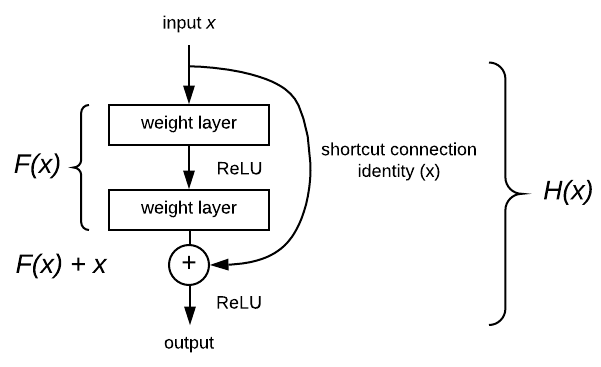
\includegraphics[width=0.65\textwidth]{figures/res-block-2}
	\caption{The original residual block design.}
	\label{fig-res-block}
\end{figure}

If we conceptualize what we want from a part of the neural network, it is to get a desired mapping $H(x)$. This can then reformulated into a residual function $F(x) = H(x) - x$. Since we are still interested in getting the desired mapping, $H(x)$ we can cast the function to be $H(x) = F(x) + x$. This might not look like much, but it showed much better error rates, compared to state-of-the-art network frameworks at the time of publication of the paper, when trained in image classification. Furthermore, it reversed the negative effect when building even deeper networks. With a ResNet, their results suggested that the deeper the network the lower the error rate. The authors hypothesized that it is easier to optimize a residual mapping, $F(x)$ than the entire desired mapping $H(x)$\cite{HeKaimingandZhangXiangyuandRenShaoqingandSun2016}.

The same authors did further experiments, among them on the function used as skip connection and the design of the residual block. The best configuration was to keep identity mapping for the shortcut, but do both activation functions, batch normalisation and ReLU, prior to the weight layers. This they called a \textit{full pre-activation}, and can be seen in figure \ref{fig-fpa-block}\cite{He2016}. Their conclusion on this is that doing batch normalisation prior to the weight layers improves regularization, which helps in reducing overfitting\footnote{Overfitting can be seen as a form of memorization. It is when a network model has specialized on predictions on specific training input, but is not learning general patterns.}.

\begin{figure}[ht]
	\centering
	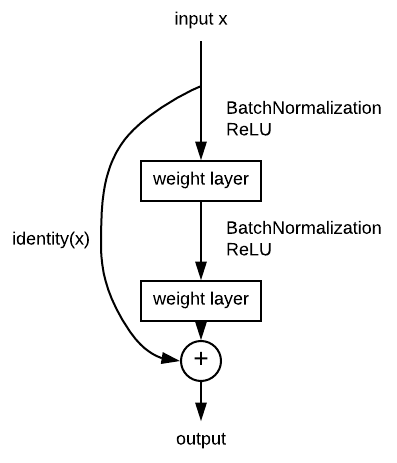
\includegraphics[width=0.45\textwidth]{figures/fpa-block-2}
	\caption{Full pre-activation residual block design.}
	\label{fig-fpa-block}
\end{figure}

In AlphaZero, DeepMind used the original residual block design. I intend to experiment with both the original and full pre-activation, to see if there are any noticeable differences in results.

\section{Network anatomy}
The anatomy of the neural network used in AlphaZero is defined in the paper \citetitle{Silver2018}\cite{Silver2018}. A basic outline can be seen in figure \ref{fig-network-structure}.

\begin{figure}[ht]
	\centering
	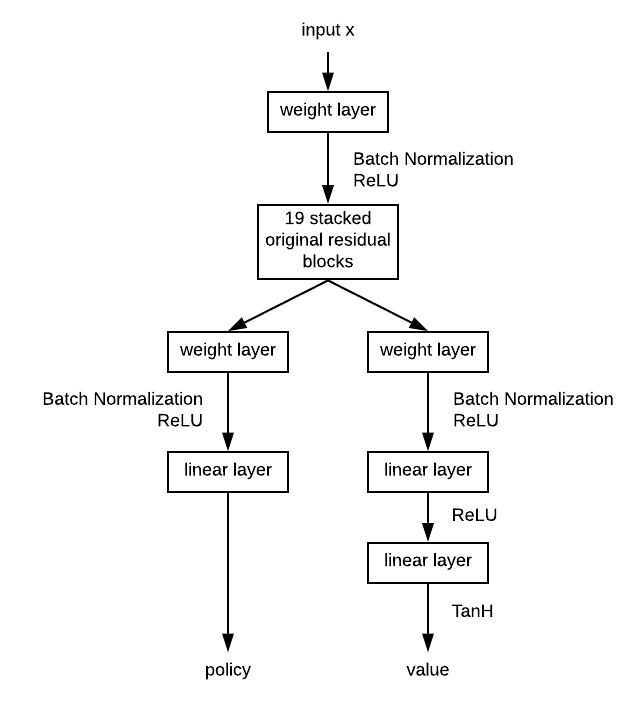
\includegraphics[width=0.75\textwidth]{figures/network-structure}
	\caption{AlphaZero's neural network structure.}
	\label{fig-network-structure}
\end{figure}

As said in the previous section, I intend to test the effect of replacing the original residual blocks with full pre-activation ones. Considering that I have less computational power at hand, it would also be interesting to measure the effect on reducing the amount of residual blocks.

\section{Monte Carlo tree search}
Roughly speaking, when Monte Carlo tree search (MCTS) was introduced, the intent was to use random sampling in a tree search, to solve decision making with the goal of getting close to an optimal action. When deciding which child node of a parent node to visit during a tree traversal, it is common to utilize the argmax\footnote{A function that returns the largest element of its input.} on the Upper Confidence Bounds (UCB1) formula applied to each child node.
\begin{equation}
v_i + c \times \sqrt[]{\frac{\ln{N}}{n_i}}
\label{ucb1}
\end{equation}

In equation \ref{ucb1}, $v_i$ is the value of the child node, $N$ is the amount of times the parent node has been visited, $n$ is the amount of times the child node has been visited, and $c$ is a constant that controls the importance the square root part of the formula. This formula serves to balance investigating parts of the tree that promises high value outcomes and parts that er under-explored. This is known as the exploitation versus exploration. The balance between the two can be adjusted by changing the value of the constant $c$.

In 2006 Hungarian computer scientist Levente Kocsis and mathematician Csaba Szepesvári published an MCTS algorithm that used random rollouts\footnote{A stochastic simulation that recursively takes random actions until a terminal state is reached.} for approximating values of nodes, and a minimax strategy for backpropagating values up the tree. The idea is that when enough random rollouts are performed it provides good approximations for the value of the different choices at the root level. This is because UCB helps building the tree asymmetrical, balancing the proportion of exploration and exploitation. This basic algorithm is known as UCB applied to trees (UCT)\cite{Kocsis2006}. In figure \ref{fig-uct} one can see an illustration of the workings of this algorithm, inspired by a similar created by Guillaume \citeauthor{Chaslot2008}\cite{Chaslot2008}.

\begin{figure}[ht]
	\centering
	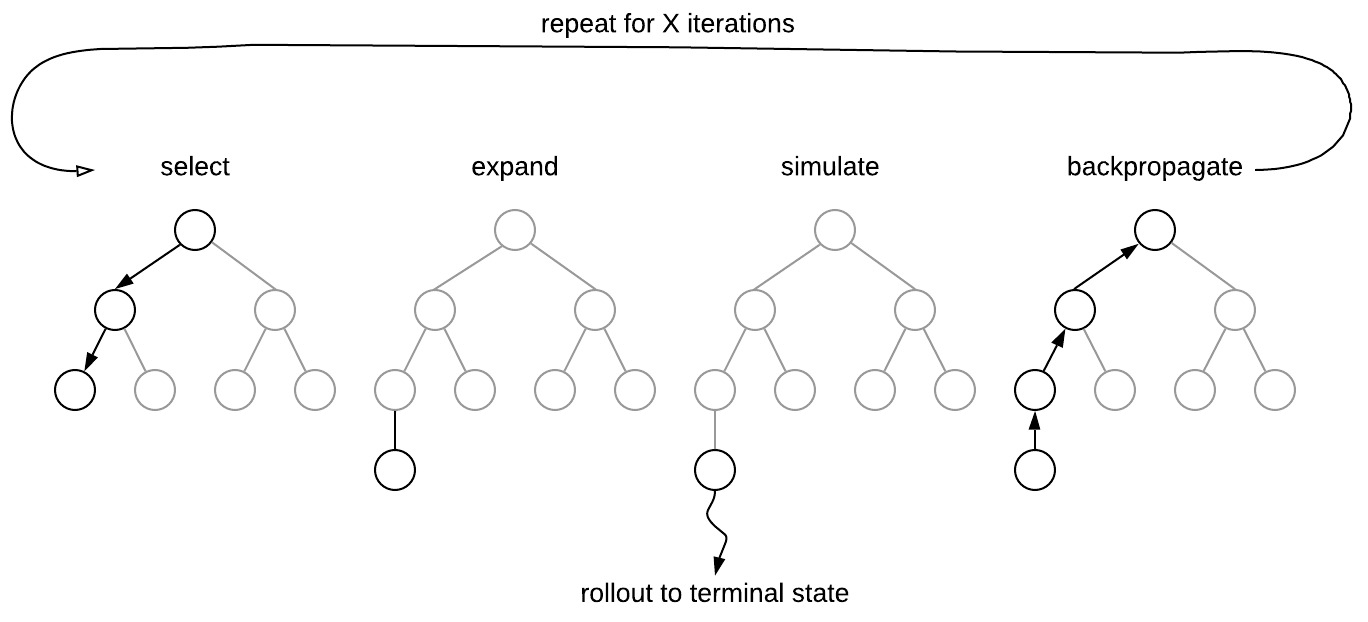
\includegraphics[width=1\textwidth]{figures/uct}
	\caption{Outline of the UCT algorithm.}
	\label{fig-uct}
\end{figure}

As shown, the algorithm works in 4 main steps. The first, \textit{select}, runs recursively with argmax and UCB1 used to choose a new parent node, until we reach a node that has at least one child node that is unvisited, or we reach a terminal state node. In \textit{expand} we return the given node if its state is terminal, otherwise we choose one of its unvisited children. In \textit{simulate} we do random rollouts till we reach a terminal state. In \textit{backpropagate}, we go back up the tree, incrementing visit count by one for all the nodes in the path, and in a minimax fashion add the value found by \textit{simulate} to a value accumulator for each node. The minimax value update is usually done by flipping the value to the perspective of the player who took a turn to reach the node. The value used in their UCB1 is the average value of a node, the accumulated value divided by the amount of visits\cite{Kocsis2006}.

\section{MCTS with neural network}
In AlphaZero a variant of Polynomial Upper Confidence Tree (PUCT) is used, which itself is variation on UCT. In addition to some changes to the UCB formula, the expand and simulate steps are combined into a single \textit{evaluate} step. In the evaluate step, the network is given a feature image array for the board state, and then returns a value for the state, and a policy vector based on prior visits to children nodes, i.e. actions taken from that state. The policy vector is then reduced to only contain the legal moves, and then applied a Softmax function. After this, the policy values are saved for the corresponding child nodes as \textit{prior} visit values.

\begin{equation}
C(p) = \log\left(\frac{1 + N_p + 19652}{19652}\right) + 1.25
\label{puct-1}
\end{equation}

\begin{equation}
U(p,c) = C(p)\times P_c\times \sqrt{\frac{N_p}{1 + N_c}}
\label{puct-2}
\end{equation}

\begin{equation}
UCB(p,c) = \frac{V_c}{N_c} + U(p,c)
\label{puct-3}
\end{equation}

Equation \ref{puct-1} corresponds to the $c$ exploration parameter from the original UCT. $N$ denotes visit count to a given node, $p$ denotes a parent node. It starts at $C \approx 1.25$ under the first iteration, and grows ever so slightly. In AlphaZero's implementation the number of MCTS iterations is set to 800, making the equation max out at $C \approx 1.29$\cite{Silver2018}. Given how small the increase is, I find it reasonable in my own implementation to set it to a constant value, thus avoiding doing the logarithmic calculations. I suspect that this difference will not hamper the exploitation versus exploration of my algorithm in any major way.

In equation \ref{puct-2}, $p$ and $c$ denotes parent and child node respectively. $P$ is the prior value from the policy output of the neural network. In equation \ref{puct-3}, $V$ denotes the accumulated value of a given node, and the entire equation gives the UCB value for the child node. It corresponds pretty well to equation \ref{ucb1}, with the main difference being the prior value added as a weight to the exploration part of the equation. Thus the neural network is informing the UCB formula used in MCTS, on how much it should weight exploration of particular nodes, and how they should be evaluated.

\section{The algorithm}
Self-play is essential for the algorithm, as it generates data for the network model to learn from. A rough outline of the running of the algorithm, imagined as if it was run sequentially, can be seen in figure \ref{fig-az-algorithm}. During self-play the AlphaZero algorithm behaves like the variant of PUCT described in the previous section, but with some random noise added to the priors of the root's children nodes, and a Softmax sampling for certain steps of each game.

\begin{figure}[ht]
	\centering
	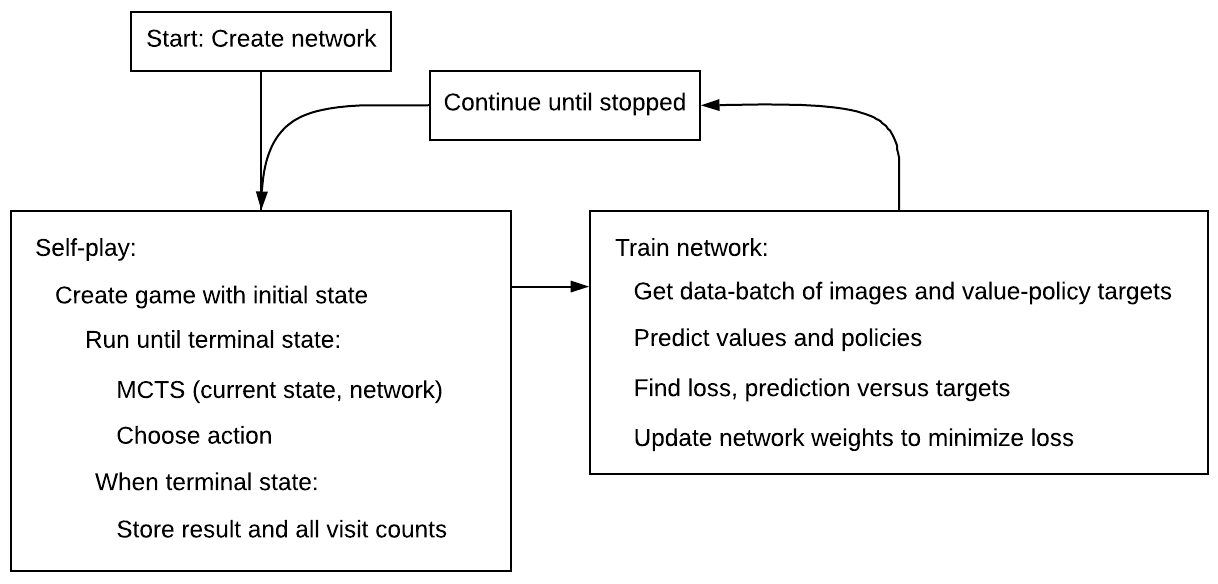
\includegraphics[width=1\textwidth]{figures/az-algorithm}
	\caption{Outline of the AlphaZero algorithm.}
	\label{fig-az-algorithm}
\end{figure}

\subsection{Self-play}
The network model's prediction might be flawed at certain steps in time, which could lead the model to converge on suboptimal action paths, and then keep training on those. Or it might be used to only seeing optimal plays, and thus will not be able to handle situations where its opponent plays suboptimal. To ensure some varieties in the game states seen by the model during training, for a certain amount of initial steps of each game, the actual action taken by the agent is chosen by a probabilistic random selection, using the result of the child node visit counts fed to a Softmax function. This random selection does almost not affect the saved data, as it does not impact the prior visit values. One could argue that it somehow flaws the value data indirectly, as the random selection might obscure who ends up winning the game. This addition to the self-play helps the network model to experience a larger state space, thus making it more robust.

For each action for the algorithm to decide, randomly generated noise is also mixed into the prior values of all the root node's children. A so-called \textit{Dirichlet distribution}, which consists of normalized gamma-distributed probabilistic values. This also diversifies the horizon of what the MCTS sees under different runs, making it possible to observe potentially stronger paths that a current network would otherwise advise against. AlphaZero uses different $\alpha$-values depending on the game; 0.3, 0.15, 0.03, for Chess, Shogi, and Go respectively. In contrast to the probabilistic random Softmax selection described in the paragraph above, this impacts both value training targets and policy training targets, because the noise affects which nodes are visited, and thus also the backpropagated values\cite{Silver2018}.

\subsection{Training}
During training, the algorithm randomly samples board states, among recorded self-play games, at randomly selected steps in time for each game. Images are created from these board states. They are then paired up with the corresponding information about the end result of the particular game, and how the visit count distribution looked for states' child nodes, after MCTS had been run on that state. The network is then tasked with making predictions on these images. A \textit{Mean Squared Error} function is applied to the predicted value and the target value. A \textit{Softmax Cross Entropy with Logits}\footnote{I have not been able to find the Tensorflow implementation of this.} function is applied to the predicted policy and the target policy. The model is then optimized with the combined loss, using Gradient Descent.

\subsection{Training targets}
In regular UCT MCTS, information about the actual game, the value of a state, is fed into the algorithm through the rollouts. In the AlphaZero algorithm the bread and butter for learning the game is training on previously played games. Here network inference is guiding the MCTS, which again provides the network information about visited root child nodes, and together with the game's end result, the utility for the terminal state of a game, forms targets the network optimizes to predict. The most important factor is this utility, as that is when information about the real game is fed into the algorithm. An illustration of this can be seen in figure\ref{fig-targets-az}.

\begin{figure}[ht]
	\centering
	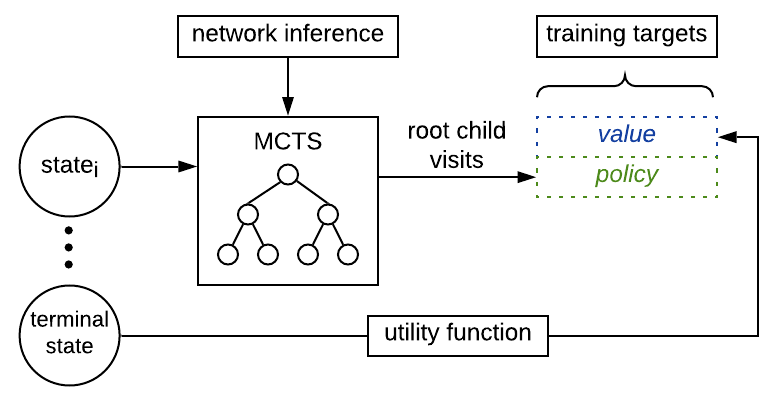
\includegraphics[width=0.6\textwidth]{figures/training-targets-az}
	\caption{Outline of how training targets are generated in the original AlphaZero approach.}
	\label{fig-targets-az}
\end{figure}

Developers from Oracle have experimented with alternative ways of giving an AlphaZero-like algorithm information about state values\cite{Abrams2018}. They test several approaches, of which I will describe two.

First, they use a game's utility function to give a value when the MCTS part reach a terminal state, thus bypassing the network, in order to get real game information. This strengthens the approximation, especially early in the run of the entire algorithm, when the network is still affected by the random weight initialization. It also indirectly helps the network, since better evaluations gives a more optimal visit count, which gives better policy for the network to optimize on. An illustration of this approach can be seen in figure \ref{fig-targets-util}.

\begin{figure}[ht]
	\centering
	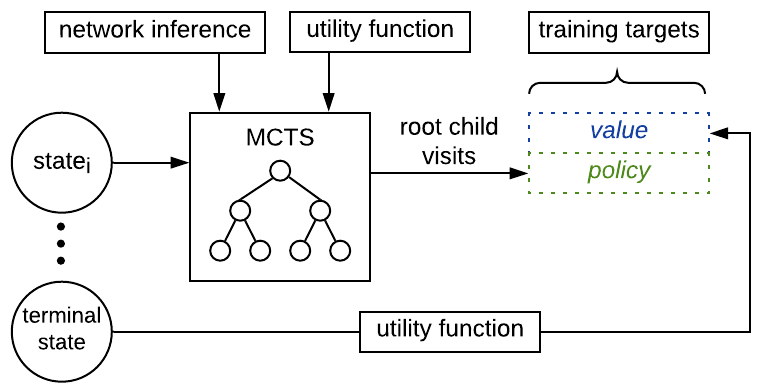
\includegraphics[width=0.6\textwidth]{figures/training-targets-util}
	\caption{Outline of the approach with utility used in MCTS evaluation at terminal states.}
	\label{fig-targets-util}
\end{figure}

Second, they change the training target value for a given board state, from the utility of a games terminal state, to the average value approximated by MCTS for the specific state in the specific game. This does not work if it is independently applied to the original AlphaZero approach, as no information about the real game utilities would then reach the algorithm. A solution like the one described in the previous paragraph is needed. This is illustrated in figure \ref{fig-targets-q}. The combined approach allows for the target value of a state to be a decimal number in the vicinity of the range $-1$ to $1$. The original approach uses discrete integer value targets, for chess -1, 0, and 1, even when a state is far from a terminal state, and one would assume there is still some uncertainty on the outcome.

\begin{figure}[ht]
	\centering
	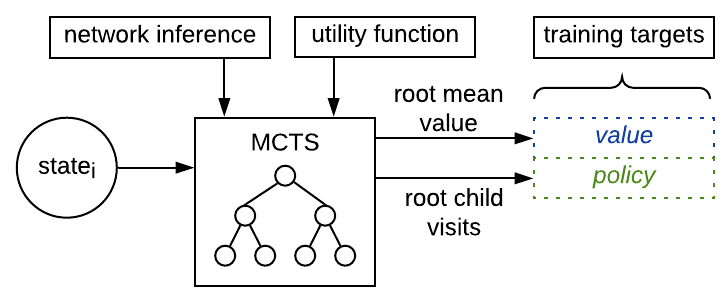
\includegraphics[width=0.6\textwidth]{figures/training-targets-q}
	\caption{Outline of the approach with both utility used in MCTS evaluation at terminal states, and the mean value at root level as value training target instead of the final game result.}
	\label{fig-targets-q}
\end{figure}

\section{Half-precision}
Half-precision floating points are of interest for deep learning, because they allow for twice the amount of variables being stored in memory, compared to single precision. But also because the new line of consumer-minded Nvidia GPUs contain Tensor cores, which allows for faster half-precision matrix operations. The hardware that will be used in this project includes such a GPU.

The most common standard for half-precision floating points is the \textit{binary16} from the IEEE Computer Society, which only uses 16 bits to represent a number\cite{Committee2008}, compared to 32 bits for a regular single precision .

Half-precision floating points take up half the amount of storage, at the cost of precision, compared to single precision floating points. For half-precision, the largest representable number is $\approx 65504$ , and the smallest positive  representable number is $\approx 0.000000059605$. In the range between these two, there is a lot of imprecision, even for the left side of the decimal separator, where not all integers in the range $0$ to $65504$ can be represented. Thus, converting from single to half precision, one can loose accuracy, as some sort of rounding occurs.

When one does an arithmetic operation on a half-precision number, that makes it smaller, but still positive, than $\approx 0.000000059605$, it will round down to $0$. If one tries to reach a number too much greater than $\approx 65504$, it will result in $\infty$. Furthermore, doing $\frac{\infty}{\infty}$, even if one or both has a negative sign, results in \textit{NaN}.

Researchers from Baidu Research and Nvidia have published a paper, where they discuss results from doing mixed-precision training for different common machine learning tasks with popular deep learning model frameworks, ResNet included\cite{Micikevicius2018}. Their mixed-precision model has a single-precision master model, on which all optimizations are done. Under each training iteration, a copy of the master, with weights, activations, and gradients being converted to half-precision. In order to avoid vanishing gradients or exploding gradients they perform a scale on them, when it is required. Additionally, all accumulations occur in single precision. Their results showed increased speed, and in some cases an increase in accuracy. The latter they speculate is because the conversion functions as a form of regularizer on the weights.
